\documentclass[12pt,letterpaper]{article}
\usepackage{preamble}
\usepackage{amsmath}
%%%%%%%%%%%%%%%%%%%%%%%%%%%%%%%%%%%%%%%%%%
%%%% Edit These for yourself
%%%%%%%%%%%%%%%%%%%%%%%%%%%%%%%%%%%%%%%%%%
\newcommand\course{Machine Learning}
\newcommand\userID{Emanuele Belli 03720425 \\ Thomas Brunner 03675118\\ Luca Corbucci 03726968}

\begin{document}.

\section*{Problem 1}

\begin{figure}[H]
\centering
  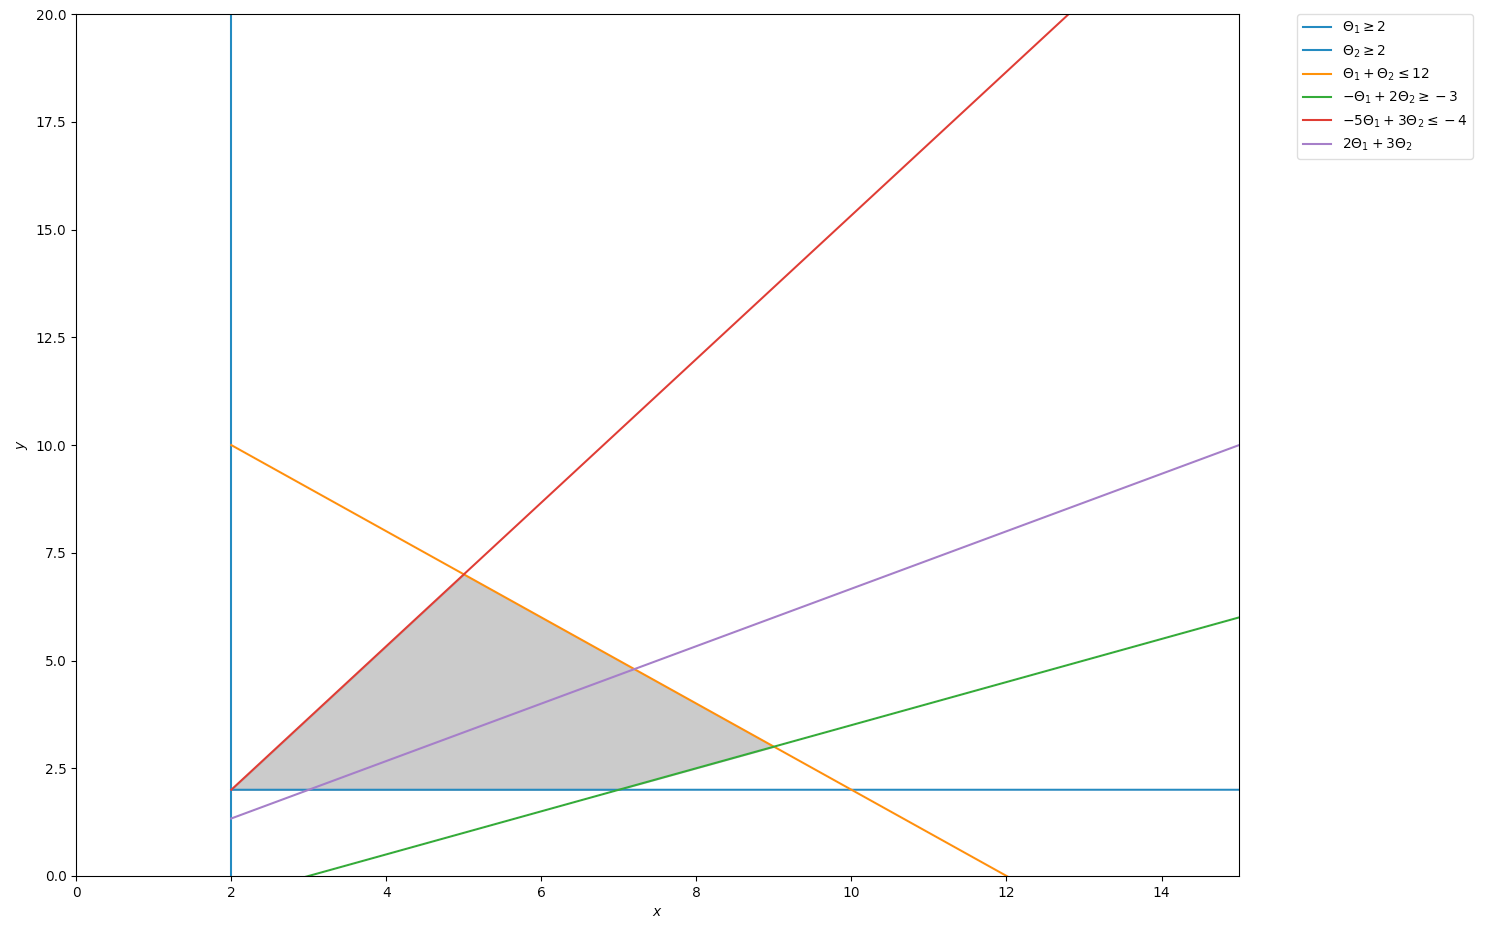
\includegraphics[width=0.8\linewidth]{Ex1.png}
\end{figure}

We can consider the vertexes of the feasible region to find the minimizer $\Theta_{min}$ and the maximizer $\Theta_{max}$.
The vertexes of the feasible region are: $(2,2)$, $(7,2)$, $(9,3)$ and $(5,7)$.

We compute the value of the objective function in each of these vertex:

\begin{itemize}
\item $(2,2)$ $->$ $f(\Theta) = -2$
\item $(7,2)$ $->$ $f(\Theta) = 8$
\item $(9,3)$ $->$ $f(\Theta) = 9$
\item $(5,7)$ $->$ $f(\Theta) = -11$
\end{itemize} 

The minimizer $\Theta_{min}$ is the vertex that produces the lower value for $f(\Theta)$: 
$$\Theta_{min} = (5,7) \ and\ Minimum\ Value = -11$$

The maximizer $\Theta_{max}$ is the vertex that produces the higher value for $f(\Theta)$: 
$$\Theta_{max} = (9,3) \ and\ Maximum\ Value = 9$$


\section*{Problem 2}

\begin{figure}[H]
\centering
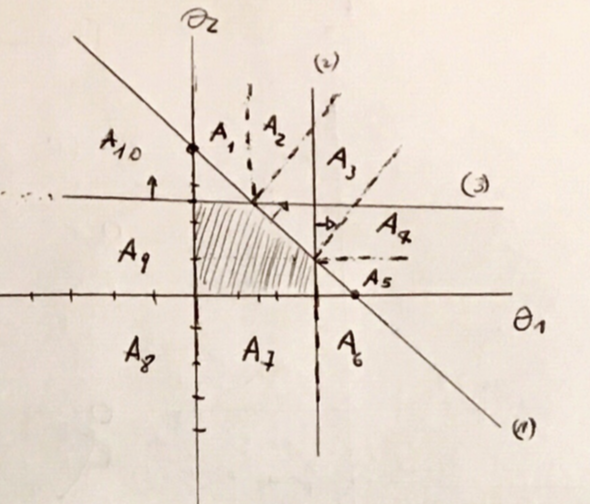
\includegraphics[width=0.6\linewidth]{pl.png}
\end{figure}



a) We can define the projections as follow:

\[ \begin{cases} 
      \Pi_X_{a,b}(p) = a+\frac{(p-a)^T(b-a)}{||b-2||_2^2}(b-a)  &     if\ p \in A_3\\
       min(max(l_i, p_i), u_i) & else
   \end{cases}
\]

If $p \not \in A_3$ we use the formula of the projection onto the box.

b) 
$$\frac{\partial }{\partial \Theta_1} = 2\Theta_1-4$$ 

$$\frac{\partial }{\partial \Theta_2} = 8\Theta_2-28$$ 

First step: 

$\Theta^1 = \Pi(\Theta^0)- \tau\nabla f(\Theta^0) =  \begin{bmatrix}2.5 \\ 1\end{bmatrix} - 0.05\begin{bmatrix}1 \\ 20\end{bmatrix} = \Pi(\begin{bmatrix}2.45 \\ 2\end{bmatrix})$
$$$$

\begin{figure}[H]
\centering
  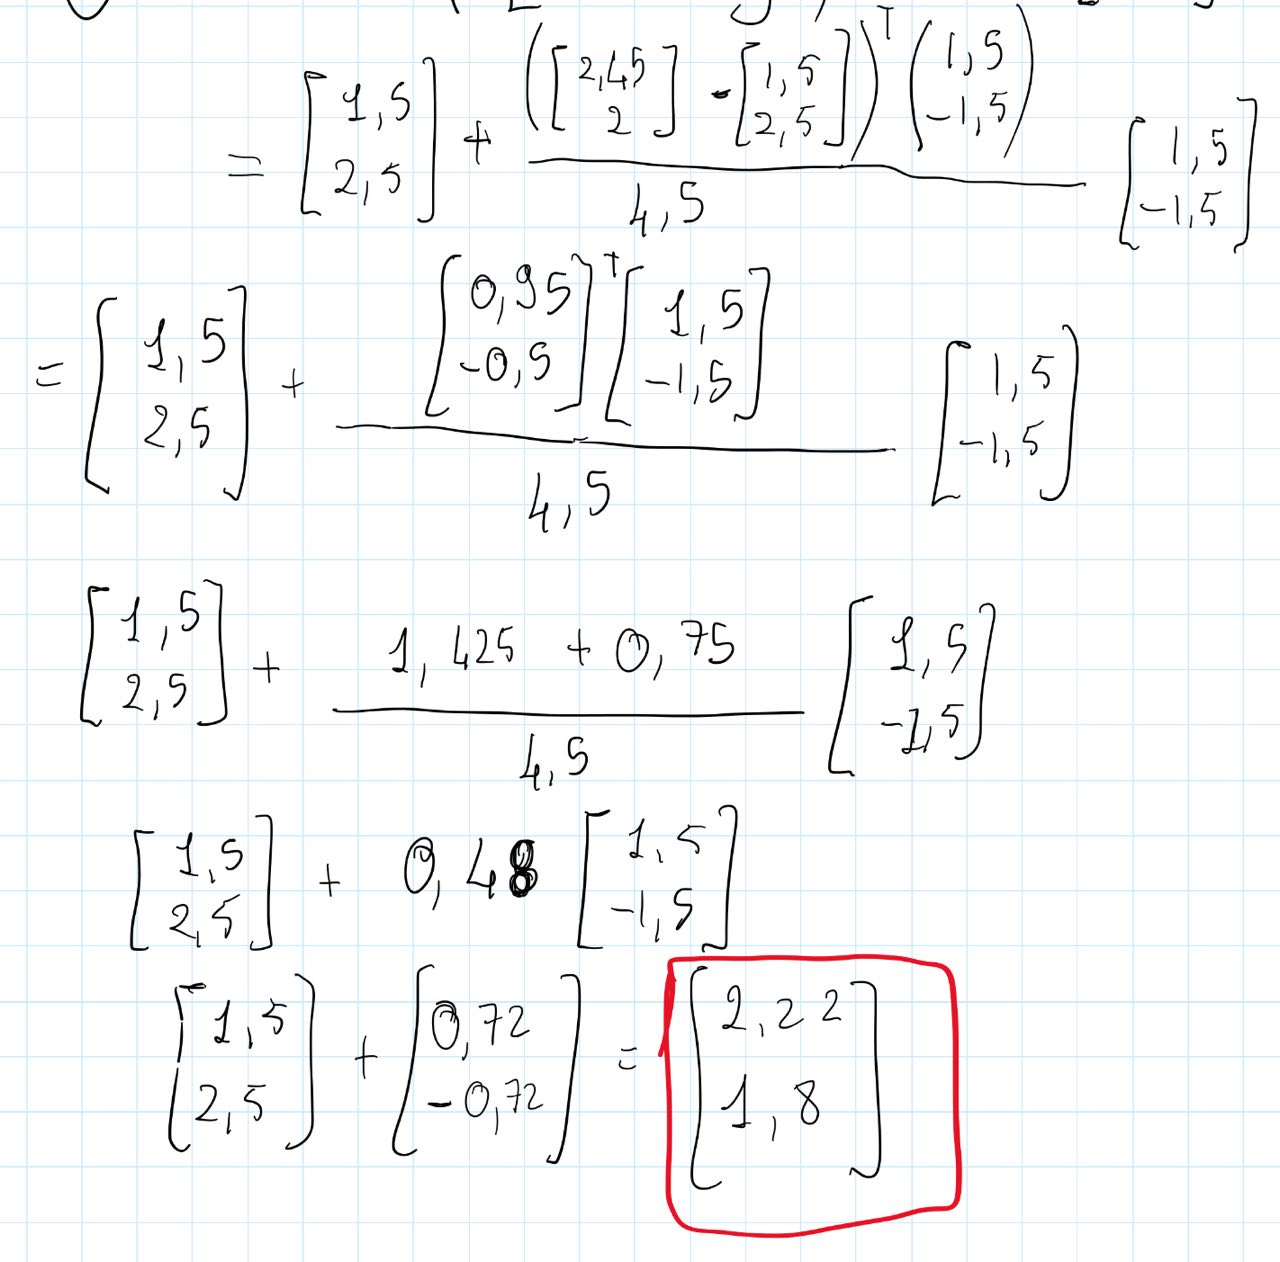
\includegraphics[width=0.6\linewidth]{1.jpeg}
\end{figure}

Second step:
\begin{figure}[H]
\centering
  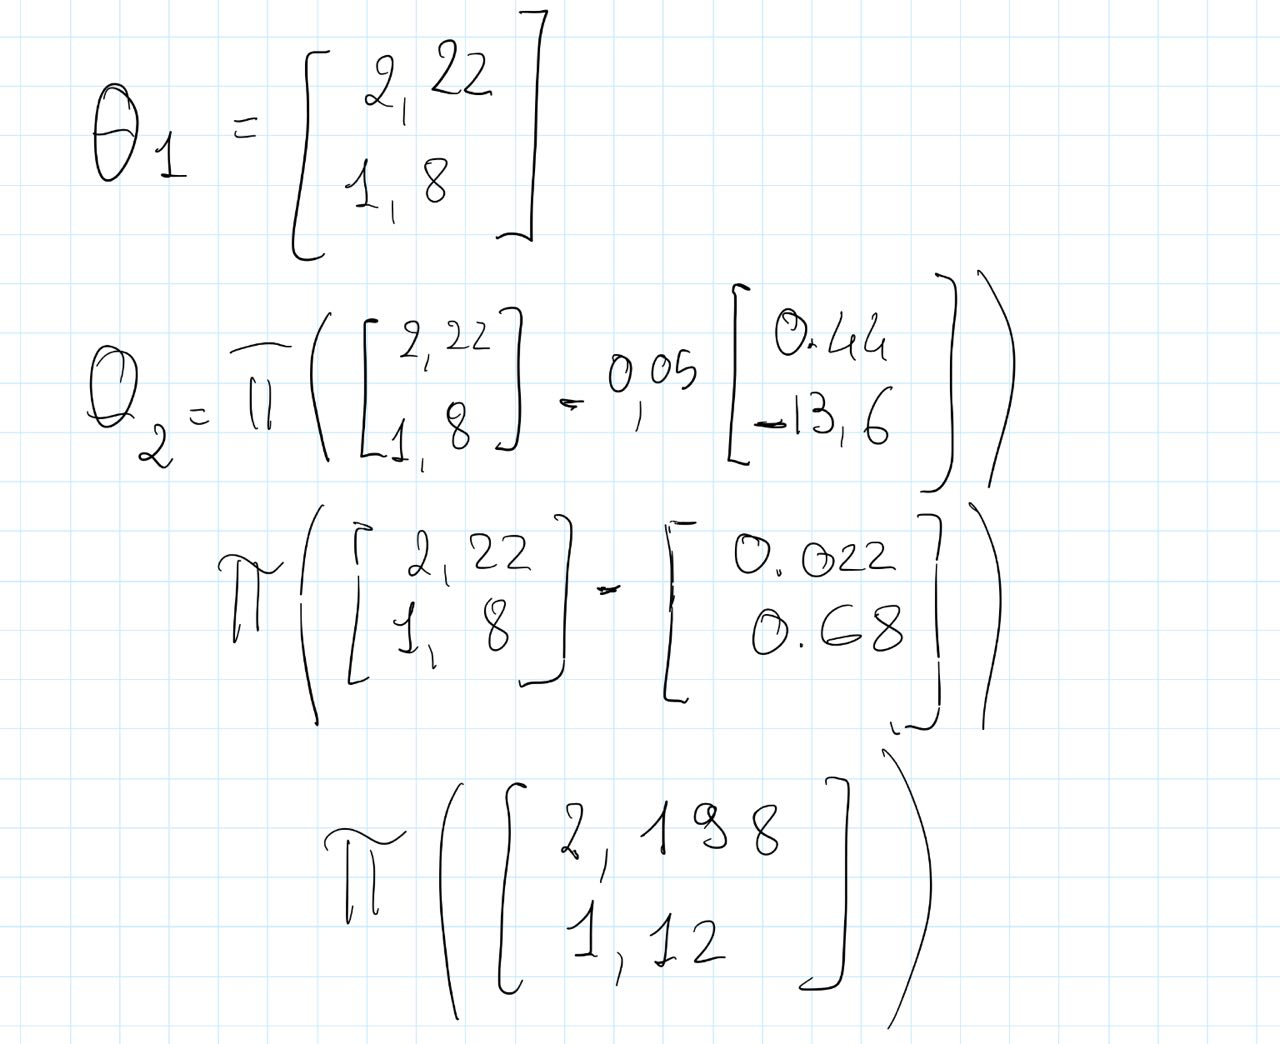
\includegraphics[width=0.6\linewidth]{2.jpeg}
  
\end{figure}

\section*{Problem 3}

a) Formulate the Lagrangian:

$$L(\Theta, \alpha) = \Theta_1 - \sqrt{3}\Theta_2 + \alpha(\Theta_1^2 + \Theta_2^2-4)$$

b) For each $\alpha \geq 0$ obtain the dual function:
$$g(\alpha) = min_\Theta L(\Theta, \alpha)$$
$$g(\alpha) = min_\Theta (\Theta_1 - \sqrt{3} \Theta_2 + \alpha(\Theta_1^2+\Theta_2^2-4))$$
Compute the partial derivatives:
$$\frac{\partial L}{\partial \Theta_1} = 1+2\alpha\Theta_1 => \Theta_1 = -\frac{1}{2\alpha}$$ 

$$\frac{\partial L}{\partial \Theta_2} = \sqrt{3}+2\alpha\Theta_2 => \Theta_2 = -\frac{\sqrt{3}}{2\alpha}$$ 

Compute $g(\alpha) = L(\Theta^*(\alpha), \alpha)$:
$$g(\alpha) = -\frac{1}{2\alpha} - \frac{3}{2\alpha} + \alpha(\frac{1}{4\alpha^2}+\frac{3}{4\alpha^2}-4) = -\frac{4}{2\alpha}+\frac{1}{\alpha} - 4\alpha = -\frac{1}{\alpha}-4\alpha$$

c) Solve the dual problem: $$maximize\ g(\alpha)$$ $$s.t.\ \alpha_i \geq 0$$

$$\frac{\partial }{\partial \alpha} = -(\alpha^{-1})-4 = \frac{1}{\alpha^2}-4=0$$

$$\alpha^2 = \frac{1}{4}$$

Possible solutions: $\alpha = +\frac{1}{2}$ and $\alpha = -\frac{1}{2}$. If we compute the second derivative we can see that we have a minimum with $\alpha = \frac{1}{2}$.

Now we can compute $\Theta_1$ and $\Theta_2$:

$$\Theta_1 = -\frac{1}{2*1/2} = -1$$
$$\Theta_2 = -\frac{\sqrt{3}}{2*1/2} = \sqrt{3}$$
 
\section*{Problem 4}

We use Slater's contions:

\begin{itemize}
\item $f_0(w) = w^tw$ which is quadratic convex 
\item $f_i(w) = -w^Ty_ix_i + (1-y_ib)$ is affine convex for all $i$
\end{itemize}

As $f_i$ is affine for all $i$, condition $(a)$ from slide 25 holds and the strong duality holds.

\end{document}
